% Options for packages loaded elsewhere
\PassOptionsToPackage{unicode}{hyperref}
\PassOptionsToPackage{hyphens}{url}
%
\documentclass[
]{article}
\usepackage{amsmath,amssymb}
\usepackage{lmodern}
\usepackage{iftex}
\ifPDFTeX
  \usepackage[T1]{fontenc}
  \usepackage[utf8]{inputenc}
  \usepackage{textcomp} % provide euro and other symbols
\else % if luatex or xetex
  \usepackage{unicode-math}
  \defaultfontfeatures{Scale=MatchLowercase}
  \defaultfontfeatures[\rmfamily]{Ligatures=TeX,Scale=1}
\fi
% Use upquote if available, for straight quotes in verbatim environments
\IfFileExists{upquote.sty}{\usepackage{upquote}}{}
\IfFileExists{microtype.sty}{% use microtype if available
  \usepackage[]{microtype}
  \UseMicrotypeSet[protrusion]{basicmath} % disable protrusion for tt fonts
}{}
\makeatletter
\@ifundefined{KOMAClassName}{% if non-KOMA class
  \IfFileExists{parskip.sty}{%
    \usepackage{parskip}
  }{% else
    \setlength{\parindent}{0pt}
    \setlength{\parskip}{6pt plus 2pt minus 1pt}}
}{% if KOMA class
  \KOMAoptions{parskip=half}}
\makeatother
\usepackage{xcolor}
\usepackage[margin=1in]{geometry}
\usepackage{graphicx}
\makeatletter
\def\maxwidth{\ifdim\Gin@nat@width>\linewidth\linewidth\else\Gin@nat@width\fi}
\def\maxheight{\ifdim\Gin@nat@height>\textheight\textheight\else\Gin@nat@height\fi}
\makeatother
% Scale images if necessary, so that they will not overflow the page
% margins by default, and it is still possible to overwrite the defaults
% using explicit options in \includegraphics[width, height, ...]{}
\setkeys{Gin}{width=\maxwidth,height=\maxheight,keepaspectratio}
% Set default figure placement to htbp
\makeatletter
\def\fps@figure{htbp}
\makeatother
\setlength{\emergencystretch}{3em} % prevent overfull lines
\providecommand{\tightlist}{%
  \setlength{\itemsep}{0pt}\setlength{\parskip}{0pt}}
\setcounter{secnumdepth}{-\maxdimen} % remove section numbering
\usepackage{fontspec}
\usepackage{polyglossia}
\setmainlanguage[babelshorthands=true]{german}
\setmainfont{merriweather}
\setsansfont{Montserrat}
\geometry{vmargin=1in,hmargin=1.25in}
\usepackage{xcolor}
\usepackage{titlesec}
\definecolor{Blue}{HTML}{2F5496}
\titleformat{\section}{\Large\sffamily\color{Blue}}{}{0pt}{}
\titleformat{\subsection}{\large\sffamily\color{Blue}}{}{0pt}{}
\titlespacing\section{0pt}{24pt plus 4pt minus 2pt}{6pt plus 2pt minus 2pt}
\titlespacing\subsection{0pt}{12pt plus 4pt minus 2pt}{2pt plus 2pt minus 2pt}
\usepackage{parskip}
\usepackage{booktabs}
\usepackage{longtable}
\usepackage{array}
\usepackage{multirow}
\usepackage{wrapfig}
\usepackage{float}
\usepackage{colortbl}
\usepackage{pdflscape}
\usepackage{tabu}
\usepackage{threeparttable}
\usepackage{threeparttablex}
\usepackage[normalem]{ulem}
\usepackage{makecell}
\usepackage{xcolor}
\usepackage{siunitx}
\newcolumntype{d}{S[input-symbols = ()]}
\ifLuaTeX
  \usepackage{selnolig}  % disable illegal ligatures
\fi
\IfFileExists{bookmark.sty}{\usepackage{bookmark}}{\usepackage{hyperref}}
\IfFileExists{xurl.sty}{\usepackage{xurl}}{} % add URL line breaks if available
\urlstyle{same} % disable monospaced font for URLs
\hypersetup{
  pdftitle={Asigment 1},
  pdfauthor={Nixon Candiales},
  hidelinks,
  pdfcreator={LaTeX via pandoc}}

\title{Asigment 1}
\author{Nixon Candiales}
\date{\today}

\begin{document}
\maketitle

\hypertarget{summary-statistics}{%
\section{Summary Statistics}\label{summary-statistics}}

Provide and discuss a table of simple summary statistics showing the
mean, standard deviation, min, and max of hospital total revenues and
uncompensated care over time.

Create a figure showing the mean hospital uncompensated care from 2000
to 2018. Show this trend separately by hospital ownership type (private
not for profit and private for profit).

\hypertarget{twfe-specification}{%
\section{TWFE Specification}\label{twfe-specification}}

Using a simple DD identification strategy, estimate the effect of
Medicaid expansion on hospital uncompensated care using a traditional
two-way fixed effects (TWFE) estimation:

\begin{equation}
y_{it} = \alpha_{i} + \gamma_{t} + \delta D_{it} + \varepsilon_{it},
(\#eq:dd)
\end{equation}

where \(D_{it}=1(E_{i}\leq t)\) in Equation @ref(eq:dd) is an indicator
set to 1 when a hospital is in a state that expanded as of year \(t\) or
earlier, \(\gamma_{t}\) denotes time fixed effects, \(\alpha_{i}\)
denotes hospital fixed effects, and \(y_{it}\) denotes the hospital's
amount of uncompensated care in year \(t\). Present four estimates from
this estimation in a table: one based on the full sample (regardless of
treatment timing); one when limiting to the 2014 treatment group (with
never treated as the control group); one when limiting to the 2015
treatment group (with never treated as the control group); and one when
limiting to the 2016 treatment group (with never treated as the control
group). Briefly explain any differences.

\hypertarget{event-study-specification}{%
\section{Event Study Specification}\label{event-study-specification}}

Estimate an ``event study'' version of the specification in part 3:
\begin{equation}
y_{it} = \alpha_{i} + \gamma_{t} +\sum_{\tau < -1} D_{it}^{\tau} \delta_{\tau} + \sum_{\tau>=0} D_{it}^{\tau} \delta_{\tau} + \varepsilon_{it},
(\#eq:event)
\end{equation} where \(D_{it}^{\tau} = 1(t-E_{i}=\tau)\) in Equation
@ref(eq:event) is essentially an interaction between the treatment dummy
and a relative time dummy. In this notation and context, \(\tau\)
denotes years relative to Medicaid expansion, so that \(\tau=-1\)
denotes the year before a state expanded Medicaid, \(\tau=0\) denotes
the year of expansion, etc. Estimate with two different samples: one
based on the full sample and one based only on those that expanded in
2014 (with never treated as the control group).

\hypertarget{sa-specification}{%
\section{SA Specification}\label{sa-specification}}

Sun and Abraham(SA) show that the \(\delta_{\tau}\) coefficients in
Equation @ref(eq:event) can be written as a non-conxvex average of all
other group-time specific average treatment effects. They propose an
interaction weighted specification:

\begin{equation}
y_{it} = \alpha_{i} + \gamma_{t} +\sum_{e} \sum_{\tau \neq -1} \left(D_{it}^{\tau} \times 1(E_{i}=e)\right) \delta_{e, \tau} + \varepsilon_{it}.
(\#eq:iwevent)
\end{equation}

Re-estimate your event study using the SA specification in Equation
@ref(eq:iwevent). Show your results for \(\hat{\delta}_{e, \tau}\) in a
Table, focusing on states with \(E_{i}=2014\), \(E_{i}=2015\), and
\(E_{i}=2016\).

Present an event study graph based on the results in part 5. Hint: you
can do this automatically in \texttt{R} with the \texttt{fixest} package
(using the \texttt{sunab} syntax for interactions), or with
\texttt{eventstudyinteract} in \texttt{Stata}. These packages help to
avoid mistakes compared to doing the tables/figures manually and also
help to get the standard errors correct.

\hypertarget{cs-specification}{%
\section{CS Specification}\label{cs-specification}}

Callaway and Sant'Anna (CS) offer a non-parametric solution that
effectively calculates a set of group-time specific differences,
\(ATT(g,t)= E[y_{it}(g) - y_{it}(\infty) | G_{i}=g]\), where \(g\)
reflects treatment timing and \(t\) denotes time. They show that under
the standard DD assumptions of parallel trends and no anticipation,
\(ATT(g,t) = E[y_{it} - y_{i, g-1} | G_{i}=g] - E[y_{it} - y_{i,g-1} | G_{i} = \infty]\),
so that \(\hat{ATT}(g,t)\) is directly estimable from sample analogs. CS
also propose aggregations of \(\hat{ATT}(g,t)\) to form an overall ATT
or a time-specific ATT (e.g., ATTs for \(\tau\) periods before/after
treatment). With this framework in mind, provide an alternative event
study using the CS estimator. Hint: check out the \texttt{did} package
in \texttt{R} or the \texttt{csdid} package in \texttt{Stata}.

\hypertarget{rr-specification}{%
\section{RR Specification}\label{rr-specification}}

Rambachan and Roth (RR) show that traditional tests of parallel
pre-trends may be underpowered, and they provide an alternative
estimator that essentially bounds the treatment effects by the size of
an assumed violation in parallel trends. One such bound RR propose is to
limit the post-treatment violation of parallel trends to be no worse
than some multiple of the pre-treatment violation of parallel trends.
Assuming linear trends, such a violation is reflected by
\[\Delta(\bar{M}) = \left\{ \delta : \forall t \geq 0, \lvert (\delta_{t+1} - \delta_{t}) - (\delta_{t} - \delta_{t-1}) \rvert \leq \bar{M} \times \max_{s<0} \lvert (\delta_{s+1} - \delta_{s}) - (\delta_{s} - \delta_{s-1}) \rvert \right\}.\]
Using the \texttt{HonestDiD} package in \texttt{R} or \texttt{Stata},
present a sensitivity plot of your CS ATT estimates using
\(\bar{M} = \{0, 0.5, 1, 1.5, 2\}\). Check out the GitHub repo
\href{https://github.com/pedrohcgs/CS_RR}{here} for some help in
combining the \texttt{HonestDiD} package with CS estimates.

\hypertarget{discussion}{%
\section{Discussion}\label{discussion}}

Discuss your findings and compare estimates from different estimators
(e.g., are your results sensitive to different specifications or
estimators? Are your results sensitive to violation of parallel trends
assumptions?).

\hypertarget{reflection}{%
\section{Reflection}\label{reflection}}

Reflect on this assignment. What did you find most challenging? What did
you find most surprising?

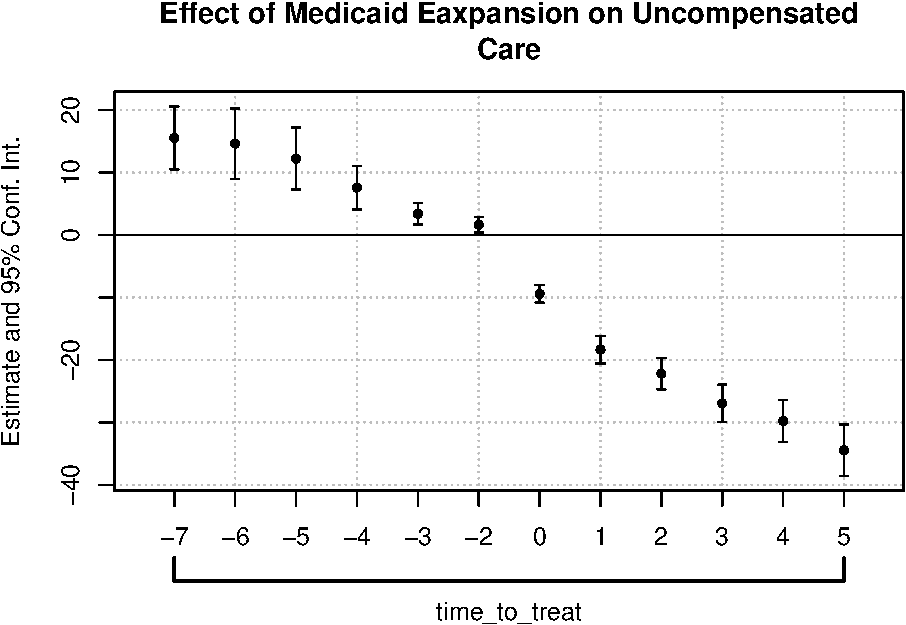
\includegraphics{Report_files/figure-latex/Figures-1.pdf}
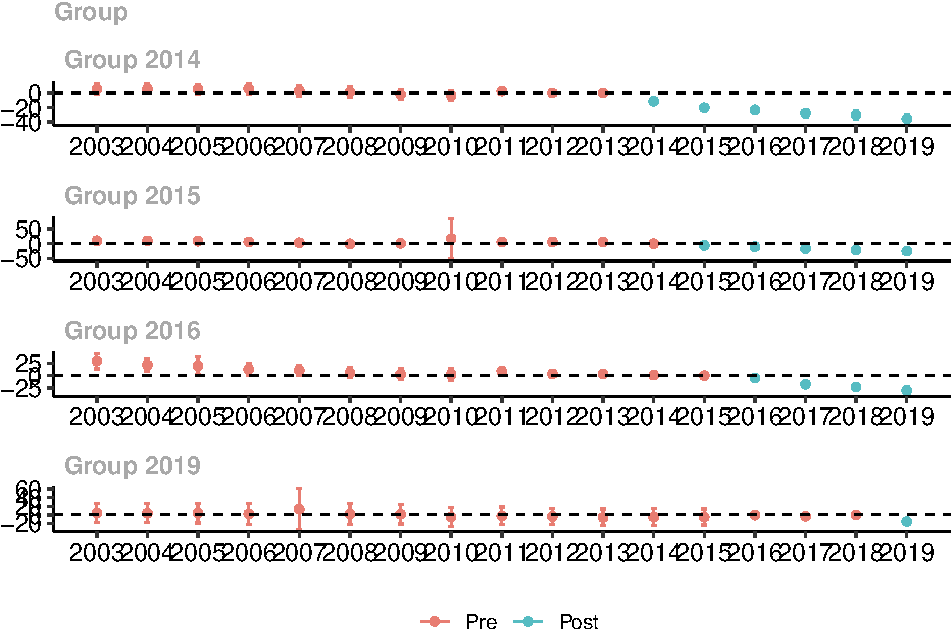
\includegraphics{Report_files/figure-latex/Figures-2.pdf}
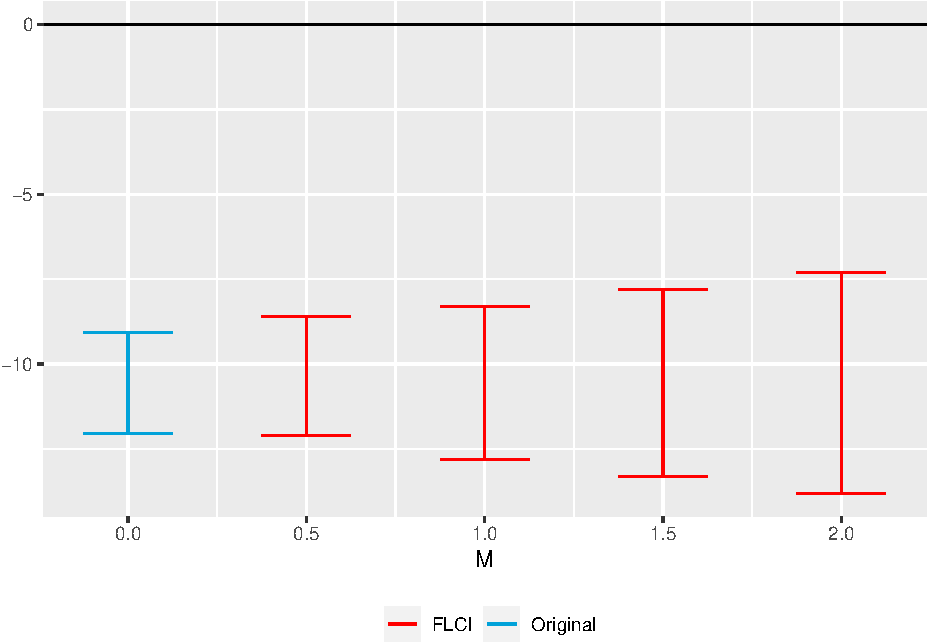
\includegraphics{Report_files/figure-latex/Figures-3.pdf}
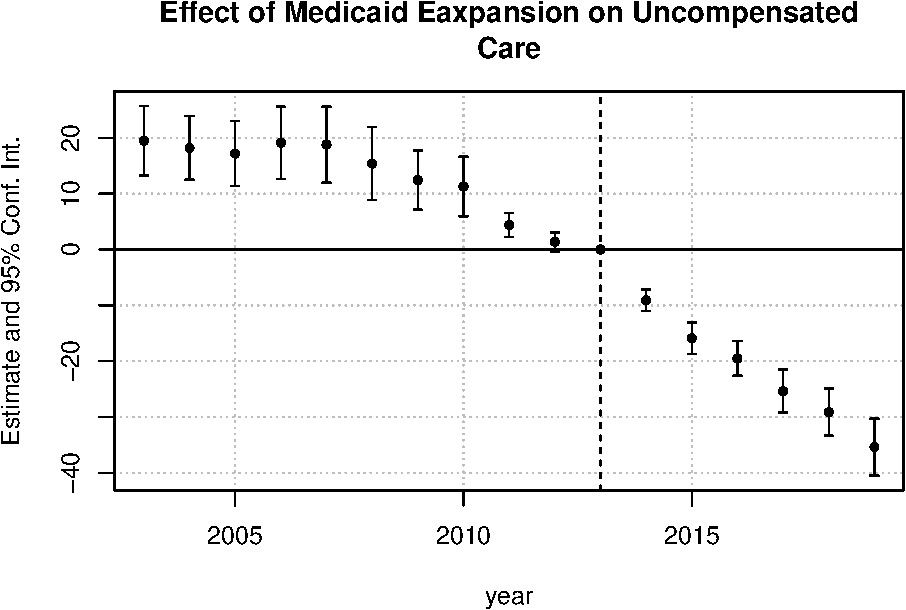
\includegraphics{Report_files/figure-latex/Figures-4.pdf}
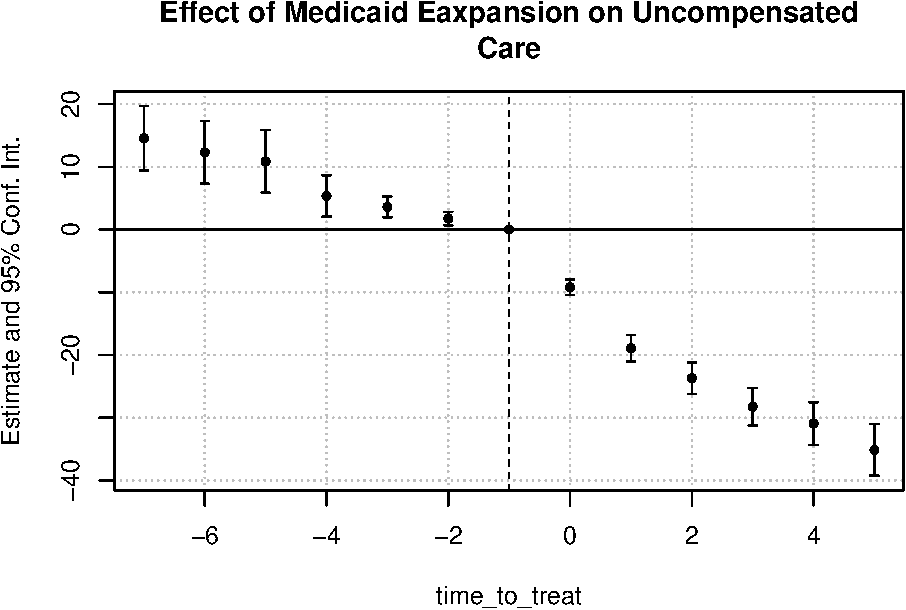
\includegraphics{Report_files/figure-latex/Figures-5.pdf}
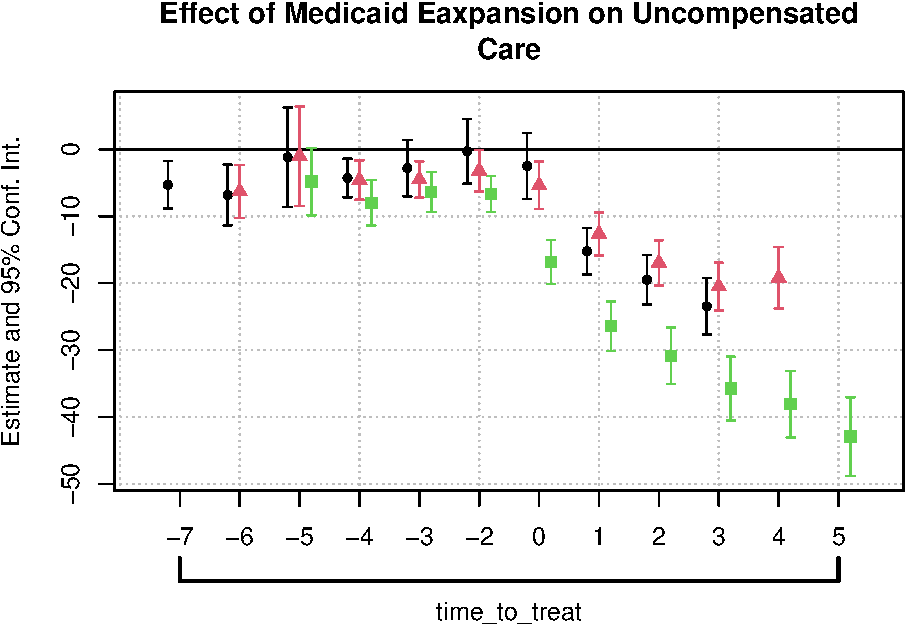
\includegraphics{Report_files/figure-latex/Figures-6.pdf}
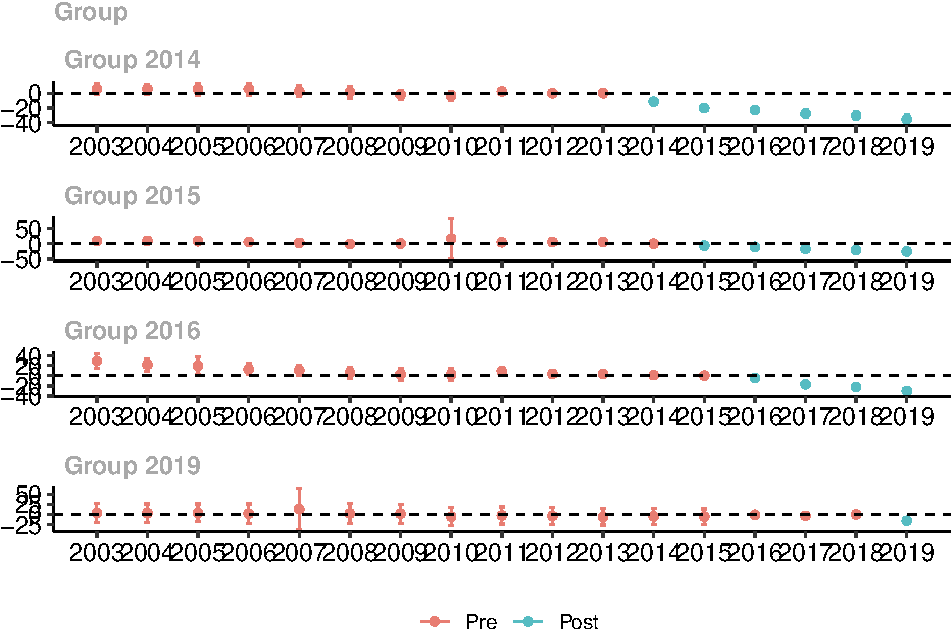
\includegraphics{Report_files/figure-latex/Figures-7.pdf}
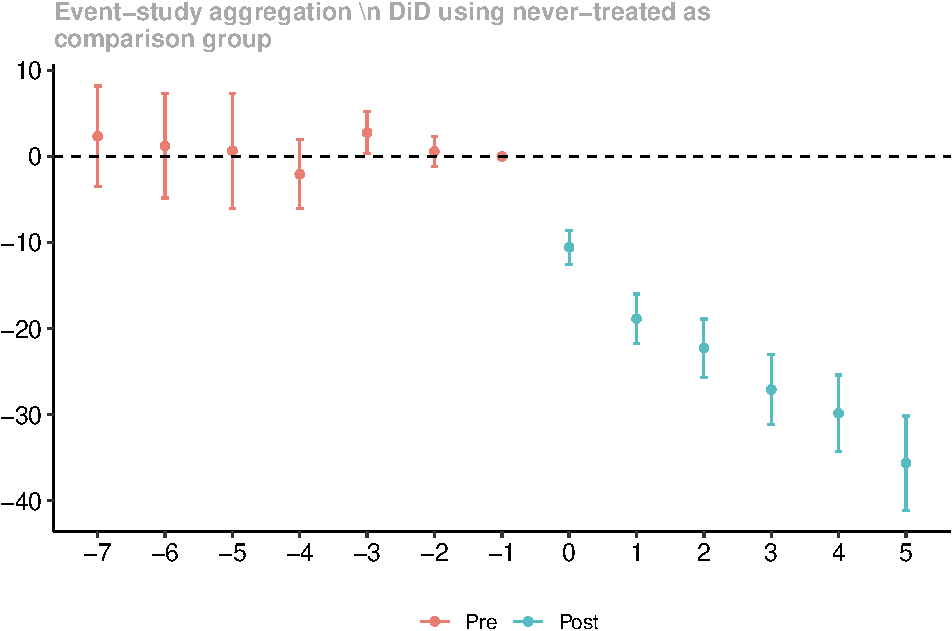
\includegraphics{Report_files/figure-latex/Figures-8.pdf}
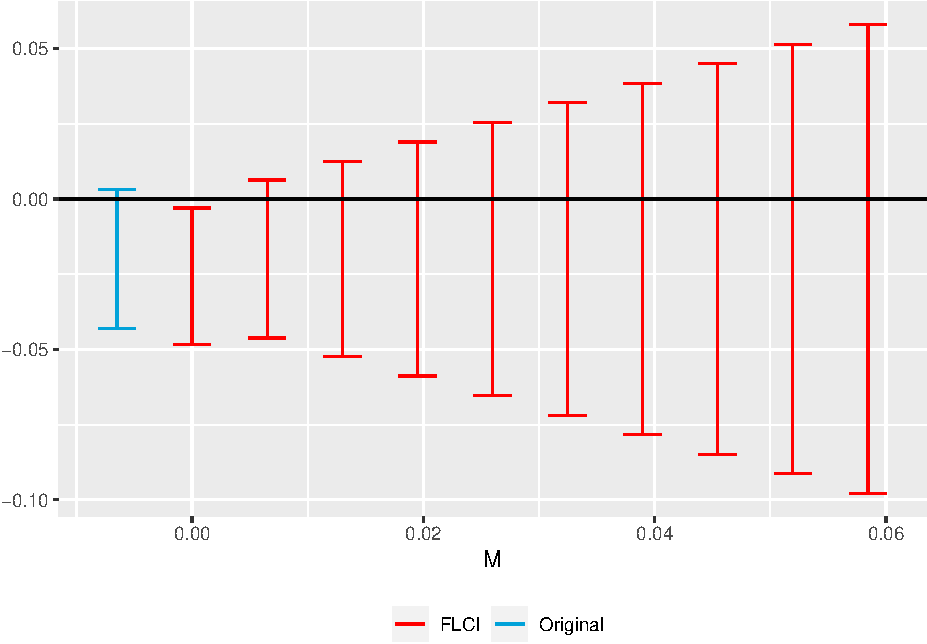
\includegraphics{Report_files/figure-latex/Figures-9.pdf}
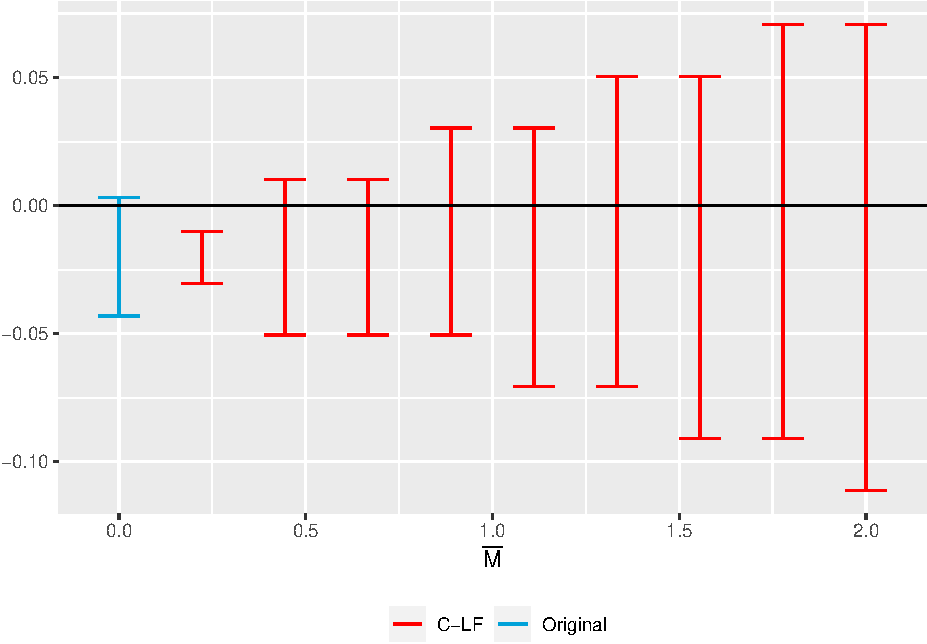
\includegraphics{Report_files/figure-latex/Figures-10.pdf}

\begin{tabular}{r|r|r|r|r|r|r|r}
\hline
unc\_care\_mean & unc\_care\_sd & unc\_care\_min & unc\_care\_max & hosp\_rev\_mean & hosp\_rev\_sd & hosp\_rev\_min & hosp\_rev\_max\\
\hline
28.16735 & 123.623 & -97.30909 & 20405.51 & 546.2998 & 960.0214 & -177.0319 & 22000.93\\
\hline
\end{tabular}

\begin{tabular}{r|r|r|r|r|r|r|r|r}
\hline
year & unc\_care\_mean & unc\_care\_sd & unc\_care\_min & unc\_care\_max & hosp\_rev\_mean & hosp\_rev\_sd & hosp\_rev\_min & hosp\_rev\_max\\
\hline
2003 & 13.55729 & 32.03610 & -0.128490 & 777.9874 & 196.3262 & 339.2561 & -1.757898 & 4722.759\\
\hline
2004 & 15.32890 & 36.66149 & 0.000001 & 820.2530 & 217.0803 & 379.3015 & 0.154394 & 5525.731\\
\hline
2005 & 17.40974 & 37.81384 & 0.000001 & 939.1340 & 237.4987 & 419.2160 & 0.000001 & 6398.554\\
\hline
2006 & 20.95880 & 47.15167 & -2.667140 & 1074.6250 & 262.1557 & 464.1907 & -0.104189 & 7784.095\\
\hline
2007 & 23.56387 & 51.27956 & 0.000001 & 1203.3748 & 285.9671 & 508.0396 & 0.063650 & 8577.046\\
\hline
2008 & 26.42960 & 57.06260 & 0.000001 & 1361.8056 & 311.2402 & 555.7333 & 0.000004 & 9293.788\\
\hline
2009 & 27.43706 & 46.41793 & 0.000001 & 583.9753 & 341.9184 & 613.2093 & 0.119236 & 9846.465\\
\hline
2010 & 29.88757 & 72.40899 & 0.000001 & 2793.9230 & 365.1954 & 647.9589 & 0.306861 & 9857.535\\
\hline
2011 & 26.76233 & 63.14211 & -54.283503 & 2059.6983 & 393.8051 & 712.2275 & -27.582223 & 10572.291\\
\hline
2012 & 29.81961 & 72.48623 & -7.440619 & 1882.6199 & 417.7530 & 765.5364 & -11.799711 & 11865.320\\
\hline
2013 & 31.89600 & 72.59600 & -4.503324 & 1652.5760 & 446.2969 & 833.9052 & 0.094880 & 12751.708\\
\hline
2014 & 31.76630 & 77.36949 & -25.850677 & 2024.8518 & 478.1198 & 905.1911 & 0.006624 & 13376.352\\
\hline
2015 & 29.81547 & 74.65024 & -0.033577 & 2054.1505 & 517.6197 & 970.8773 & 0.009368 & 14143.533\\
\hline
2016 & 35.52159 & 310.04681 & -0.018982 & 20405.5142 & 562.2181 & 1070.3765 & -177.031923 & 15618.749\\
\hline
2017 & 33.37365 & 87.34864 & -0.027988 & 2733.5950 & 603.0033 & 1167.5586 & 0.124513 & 16863.431\\
\hline
2018 & 35.88876 & 90.47501 & -0.064101 & 2606.3455 & 651.7126 & 1283.8391 & 0.282914 & 18677.245\\
\hline
2019 & 39.77855 & 99.47749 & -97.309089 & 2648.2579 & 706.4571 & 1419.7912 & 0.000003 & 22000.932\\
\hline
\end{tabular}

\begin{table}[H] \centering 
  \caption{Two Way Fixed Effect Model} 
  \label{table-3} 
\begin{tabular}{@{\extracolsep{5pt}}lcccc} 
\\[-1.8ex]\hline 
\hline \\[-1.8ex] 
 & \multicolumn{4}{c}{\textit{Dependent variable:}} \\ 
\cline{2-5} 
\\[-1.8ex] & \multicolumn{4}{c}{unc\_care} \\ 
 & M1 & M2 & M3 &  \\ 
\hline \\[-1.8ex] 
 Treatment & $-$28.191$^{***}$ & $-$26.243$^{***}$ & $-$12.003$^{***}$ & $-$12.424$^{***}$ \\ 
  & (1.883) & (1.795) & (1.811) & (1.543) \\ 
  & & & & \\ 
\hline \\[-1.8ex] 
Observations & 79,557 & 79,557 & 79,557 & 79,557 \\ 
R$^{2}$ & 0.699 & 0.697 & 0.690 & 0.690 \\ 
Adjusted R$^{2}$ & 0.675 & 0.673 & 0.665 & 0.665 \\ 
Residual Std. Error (df = 73725) & 39.701 & 39.829 & 40.304 & 40.313 \\ 
\hline 
\hline \\[-1.8ex] 
\textit{Note:}  & \multicolumn{4}{r}{$^{*}$p$<$0.1; $^{**}$p$<$0.05; $^{***}$p$<$0.01} \\ 
\end{tabular} 
\end{table}

\begin{table}

\caption{\label{tab:table-4}Two Way Fixed Effects long format}
\centering
\begin{tabular}[t]{lcccc}
\toprule
  & d & d\_14 & d\_15 & d\_16\\
\midrule
Treatment & \num{-28.191}*** & \num{-26.243}*** & \num{-12.003}*** & \num{-12.424}***\\
 & (\num{1.883}) & (\num{1.795}) & (\num{1.811}) & (\num{1.543})\\
\midrule
Num.Obs. & \num{79557} & \num{79557} & \num{79557} & \num{79557}\\
R2 & \num{0.699} & \num{0.697} & \num{0.690} & \num{0.690}\\
R2 Adj. & \num{0.675} & \num{0.673} & \num{0.665} & \num{0.665}\\
AIC & \num{817139.6} & \num{817654.2} & \num{819537.5} & \num{819575.0}\\
BIC & \num{871294.5} & \num{871809.1} & \num{873692.4} & \num{873729.9}\\
RMSE & \num{38.22} & \num{38.34} & \num{38.80} & \num{38.81}\\
Std.Errors & by: pn & by: pn & by: pn & by: pn\\
\bottomrule
\multicolumn{5}{l}{\rule{0pt}{1em}+ p $<$ 0.1, * p $<$ 0.05, ** p $<$ 0.01, *** p $<$ 0.001}\\
\end{tabular}
\end{table}

\begin{table}

\caption{\label{tab:table-4}Event Study Common Treatment}
\centering
\begin{tabular}[t]{lc}
\toprule
  & Model 1\\
\midrule
year = 2003 × treated & \num{19.485}***\\
 & (\num{3.164})\\
year = 2004 × treated & \num{18.189}***\\
 & (\num{2.908})\\
year = 2005 × treated & \num{17.172}***\\
 & (\num{2.965})\\
year = 2006 × treated & \num{19.119}***\\
 & (\num{3.292})\\
year = 2007 × treated & \num{18.782}***\\
 & (\num{3.478})\\
year = 2008 × treated & \num{15.392}***\\
 & (\num{3.328})\\
year = 2009 × treated & \num{12.430}***\\
 & (\num{2.711})\\
year = 2010 × treated & \num{11.285}***\\
 & (\num{2.717})\\
year = 2011 × treated & \num{4.376}***\\
 & (\num{1.106})\\
year = 2012 × treated & \num{1.371}\\
 & (\num{0.873})\\
year = 2014 × treated & \num{-9.102}***\\
 & (\num{0.987})\\
year = 2015 × treated & \num{-15.893}***\\
 & (\num{1.431})\\
year = 2016 × treated & \num{-19.503}***\\
 & (\num{1.585})\\
year = 2017 × treated & \num{-25.378}***\\
 & (\num{1.959})\\
year = 2018 × treated & \num{-29.139}***\\
 & (\num{2.155})\\
year = 2019 × treated & \num{-35.394}***\\
 & (\num{2.603})\\
\midrule
Num.Obs. & \num{79557}\\
AIC & \num{804621.4}\\
BIC & \num{804779.2}\\
RMSE & \num{38.01}\\
Std.Errors & by: pn\\
FE: pn & X\\
FE: year & X\\
\bottomrule
\multicolumn{2}{l}{\rule{0pt}{1em}+ p $<$ 0.1, * p $<$ 0.05, ** p $<$ 0.01, *** p $<$ 0.001}\\
\end{tabular}
\end{table}

\begin{table}

\caption{\label{tab:table-4}Even Study Staggered}
\centering
\begin{tabular}[t]{lc}
\toprule
  & Model 1\\
\midrule
time\_to\_treat = -7 × treated & \num{5.137}***\\
 & (\num{1.412})\\
time\_to\_treat = -6 × treated & \num{4.920}**\\
 & (\num{1.502})\\
time\_to\_treat = -5 × treated & \num{2.254}\\
 & (\num{1.551})\\
time\_to\_treat = -4 × treated & \num{-1.602}\\
 & (\num{1.308})\\
time\_to\_treat = -3 × treated & \num{-2.416}*\\
 & (\num{1.027})\\
time\_to\_treat = -2 × treated & \num{-0.141}\\
 & (\num{0.578})\\
time\_to\_treat = 0 × treated & \num{8.151}***\\
 & (\num{1.599})\\
time\_to\_treat = 1 × treated & \num{-16.830}***\\
 & (\num{1.009})\\
time\_to\_treat = 2 × treated & \num{-22.370}***\\
 & (\num{1.256})\\
time\_to\_treat = 3 × treated & \num{-27.793}***\\
 & (\num{1.537})\\
time\_to\_treat = 4 × treated & \num{-30.231}***\\
 & (\num{1.738})\\
time\_to\_treat = 5 × treated & \num{-33.524}***\\
 & (\num{2.060})\\
\midrule
Num.Obs. & \num{79557}\\
AIC & \num{805085.8}\\
BIC & \num{805206.5}\\
RMSE & \num{38.12}\\
Std.Errors & by: pn\\
FE: pn & X\\
FE: year & X\\
\bottomrule
\multicolumn{2}{l}{\rule{0pt}{1em}+ p $<$ 0.1, * p $<$ 0.05, ** p $<$ 0.01, *** p $<$ 0.001}\\
\end{tabular}
\end{table}

\begin{table}

\caption{\label{tab:table-4}SA especification}
\centering
\begin{tabular}[t]{lccc}
\toprule
  & mod.sa.2016 & mod.sa.2015 & mod.sa.2014\\
\midrule
time\_to\_treat = -7 & \num{-5.298}** &  & \\
 & (\num{1.806}) &  & \\
time\_to\_treat = -6 & \num{-6.820}** & \num{-6.301}** & \\
 & (\num{2.306}) & (\num{2.025}) & \\
time\_to\_treat = -5 & \num{-1.181} & \num{-1.023} & \num{-4.815}+\\
 & (\num{3.792}) & (\num{3.790}) & (\num{2.575})\\
time\_to\_treat = -4 & \num{-4.281}** & \num{-4.591}** & \num{-7.985}***\\
 & (\num{1.474}) & (\num{5.908}) & (\num{1.733})\\
time\_to\_treat = -3 & \num{-2.801} & \num{-4.501}** & \num{-6.371}***\\
 & (\num{2.155}) & (\num{2.097}) & (\num{1.529})\\
time\_to\_treat = -2 & \num{-0.286} & \num{-3.207}* & \num{-6.684}***\\
 & (\num{2.473}) & (\num{1.384}) & (\num{1.369})\\
time\_to\_treat = 0 & \num{-2.493} & \num{-5.394}** & \num{-16.855}***\\
 & (\num{2.524}) & (\num{1.278}) & (\num{1.673})\\
time\_to\_treat = 1 & \num{-15.240}*** & \num{-12.623}*** & \num{-26.405}***\\
 & (\num{1.783}) & (\num{1.921}) & (\num{1.890})\\
time\_to\_treat = 2 & \num{-19.497}*** & \num{-16.957}*** & \num{-30.859}***\\
 & (\num{1.880}) & (\num{2.156}) & (\num{2.158})\\
time\_to\_treat = 3 & \num{-23.461}*** & \num{-20.513}*** & \num{-35.758}***\\
 & (\num{2.161}) & (\num{2.128}) & (\num{2.431})\\
time\_to\_treat = 4 &  & \num{-19.194}*** & \num{-38.103}***\\
 &  & (\num{5.484}) & (\num{2.538})\\
time\_to\_treat = 5 &  &  & \num{-42.934}***\\
 &  &  & (\num{3.003})\\
\midrule
Num.Obs. & \num{79557} & \num{79557} & \num{79557}\\
AIC & \num{807862.7} & \num{807729.3} & \num{804897.4}\\
BIC & \num{807964.8} & \num{807831.4} & \num{804999.5}\\
RMSE & \num{38.79} & \num{38.76} & \num{38.07}\\
Std.Errors & by: pn & by: pn & by: pn\\
FE: pn & X & X & X\\
FE: year & X & X & X\\
\bottomrule
\multicolumn{4}{l}{\rule{0pt}{1em}+ p $<$ 0.1, * p $<$ 0.05, ** p $<$ 0.01, *** p $<$ 0.001}\\
\end{tabular}
\end{table}

\begin{table}

\caption{\label{tab:table-4}CS specification}
\centering
\begin{tabular}[t]{lc}
\toprule
  & Model 1\\
\midrule
ATT(2014,2012) & \num{0.501}\\
 & (\num{0.852})\\
ATT(2014,2013) & \num{0.000}\\
ATT(2014,2014) & \num{-10.982}\\
 & (\num{2.115})\\
ATT(2014,2015) & \num{-19.827}\\
 & (\num{3.640})\\
ATT(2014,2016) & \num{-22.794}\\
 & (\num{4.308})\\
ATT(2014,2017) & \num{-27.690}\\
 & (\num{5.275})\\
ATT(2014,2018) & \num{-30.212}\\
 & (\num{6.353})\\
ATT(2014,2019) & \num{-35.792}\\
 & (\num{8.740})\\
ATT(2015,2012) & \num{6.244}\\
 & (\num{2.258})\\
ATT(2015,2013) & \num{5.781}\\
 & (\num{1.853})\\
ATT(2015,2014) & \num{0.000}\\
ATT(2015,2015) & \num{-5.401}\\
 & (\num{2.480})\\
ATT(2015,2016) & \num{-9.522}\\
 & (\num{2.284})\\
ATT(2015,2017) & \num{-16.522}\\
 & (\num{3.369})\\
ATT(2015,2018) & \num{-20.673}\\
 & (\num{4.328})\\
ATT(2015,2019) & \num{-25.534}\\
 & (\num{6.872})\\
ATT(2016,2012) & \num{3.523}\\
 & (\num{4.775})\\
ATT(2016,2013) & \num{2.544}\\
 & (\num{4.380})\\
ATT(2016,2014) & \num{0.879}\\
 & (\num{1.537})\\
ATT(2016,2015) & \num{0.000}\\
ATT(2016,2016) & \num{-4.752}\\
 & (\num{1.310})\\
ATT(2016,2017) & \num{-18.249}\\
 & (\num{4.751})\\
ATT(2016,2018) & \num{-23.546}\\
 & (\num{5.796})\\
ATT(2016,2019) & \num{-31.190}\\
 & (\num{7.334})\\
ATT(2019,2012) & \num{-2.711}\\
 & (\num{11.516})\\
ATT(2019,2013) & \num{-4.623}\\
 & (\num{11.396})\\
ATT(2019,2014) & \num{-3.978}\\
 & (\num{9.381})\\
ATT(2019,2015) & \num{-3.711}\\
 & (\num{6.772})\\
ATT(2019,2016) & \num{-0.441}\\
 & (\num{4.826})\\
ATT(2019,2017) & \num{-3.331}\\
 & (\num{3.430})\\
ATT(2019,2018) & \num{0.000}\\
ATT(2019,2019) & \num{-15.267}\\
 & (\num{3.390})\\
\midrule
Num.Obs. & \num{51}\\
Std.Errors & by: state\_id\\
ngroup & \num{4.000}\\
ntime & \num{8.000}\\
control.group & nevertreated\\
est.method & dr\\
\bottomrule
\end{tabular}
\end{table}

\begin{table}

\caption{\label{tab:table-4}CS specification Event Study}
\centering
\begin{tabular}[t]{lc}
\toprule
  & Model 1\\
\midrule
ATT(-5) & \num{-3.978}\\
 & (\num{9.229})\\
ATT(-4) & \num{-0.094}\\
 & (\num{5.270})\\
ATT(-3) & \num{3.277}\\
 & (\num{3.012})\\
ATT(-2) & \num{0.764}\\
 & (\num{0.947})\\
ATT(-1) & \num{0.000}\\
ATT(0) & \num{-10.375}\\
 & (\num{2.090})\\
ATT(1) & \num{-18.762}\\
 & (\num{3.406})\\
ATT(2) & \num{-22.253}\\
 & (\num{4.142})\\
ATT(3) & \num{-27.251}\\
 & (\num{5.016})\\
ATT(4) & \num{-29.744}\\
 & (\num{6.283})\\
ATT(5) & \num{-35.792}\\
 & (\num{8.920})\\
\midrule
Num.Obs. & \num{51}\\
Std.Errors & by: state\_id\\
type & dynamic\\
ngroup & \num{4.000}\\
ntime & \num{8.000}\\
control.group & nevertreated\\
est.method & dr\\
\bottomrule
\end{tabular}
\end{table}

\end{document}
